\documentclass{letter}

\usepackage[left=0.75in, right=0.75in, top=1.1in, bottom=0.75in]{geometry}
\usepackage{fancyhdr, amsmath, amssymb, mathtools, xcolor, graphicx, listings, mathpazo}
\graphicspath{{.}}

\pagestyle{fancy}
\fancyhf{}
\rhead{Page \thepage}
\chead{AMSC808N Final Exam Problem 2}
\lhead{Tyler Hoffman}
\setlength{\headsep}{0.2in}

\newcounter{problem}
\newcounter{subproblem}[problem]
\newcounter{solution}

\renewcommand{\thesubproblem}{(\alph{subproblem})}

\newcommand{\Problem}[2]{%
	\stepcounter{problem}%
	\leftskip=0pt%
	\theproblem.~\textbf{{#1.}} #2 \par%
}

\newcommand{\Subproblem}[1]{%
	\stepcounter{subproblem}%
	\leftskip=15pt%
	\thesubproblem~ #1 \par%
}

\newcommand{\Solution}[1]{%
	\textbf{Solution.} #1 \par%
}

\newcommand{\Due}[1]{\textbf{Due: #1} \par}

\newcommand{\UNFINISHED}{\textbf{\color{red} UNFINISHED}}
\newcommand{\CHECK}{\textbf{\color{orange} CHECK ME}}

\newcommand{\iu}{{i\mkern1mu}}
\newcommand{\T}{\intercal}
\newcommand{\R}{\mathbb{R}}

\DeclareMathOperator{\diag}{diag}
\DeclareMathOperator{\rank}{rank}
\DeclareMathOperator{\nul}{nul}
\DeclareMathOperator{\tr}{tr}

\usepackage{hyperref}
\begin{document}
    \Due{21 Dec 2020}

    The code for this problem can be found \UNFINISHED

    \Problem{Epidemic creation}{Consider a SIR model for propagating infectious disease over a random graph with degree distribution $\{p_k\}$ such that there exists a giant component. Let $T$ be the probability for any given edge to transmit the infection. What is the critical transmissibility $T_c$ such that if $T < T_c$ an epidemic cannot occur and if $T > T_c$ an epidemic can occur? Express it via $\kappa := \langle k^2 \rangle / \langle k \rangle$, the ratio of the second and first moments of the original graph. 
    
    Assume that if $T > T_c$ an epidemic is possible. Suppose that we vaccinate a fraction $v$ of randomly selected nodes. Derive an expression for the critical fraction of nodes $v_c$ such that if $v > v_c$, an epidemic cannot occur, but if $v < v_c$, an epidemic can occur.}
    \Solution{As we saw from Newman (2002) in class, we know that for a random graph with degree distribution $\{p_k\}$ the value $T_c$ is \begin{align*}
        T_c = \frac{\sum_{k = 1}^\infty kp_k}{\sum_{k = 2}^\infty k(k - 1)p_k} = \frac{\langle k \rangle}{\sum_{k = 2}^\infty k^2p_k - \sum_{k = 2}^\infty kp_k} = \frac{\langle k \rangle}{\langle k^2 \rangle + p_1 - \langle k \rangle - p_1} = \frac{\langle k \rangle}{\langle k^2 \rangle - \langle k \rangle} = \frac{1}{\kappa - 1}.
    \end{align*} Next, we compute the probability of transmission in the graph with vaccinated nodes. \begin{align*}
        P(\text{transmission}) &= P(\text{transmission}|\text{vaccinated})P(\text{vaccinated}) + P(\text{transmission}|\text{unvaccinated})P(\text{unvaccinated}) \\
        &= (1-v)P(\text{transmission}|\text{unvaccinated}) \\
        &= (1-v)T.
    \end{align*} Since vaccinated nodes cannot be infected, the first term drops out. Since the fraction of nodes that are vaccinated is $v$, the probability that a randomly selected node is vaccinated is $v$. Finally, $P(\text{transmission}|\text{unvaccinated})$ is simply the regular transmission process we used before with probability $T$. We can now continue as before, following Newman (2002) and the lecture notes. The probability that a vertex with degree $k$ has $m$ transmitting edges is $\binom{k}{m}(1-v)^mT^m(1-(1-v)T)^{k-m}$ and therefore the probability that an arbitrary vertex has $m$ transmitting edges is \begin{align*}
        \sum_{k=m}^\infty p_k \binom{k}{m}(1-v)^mT^m(1-(1-v)T)^{k-m}.
    \end{align*} The generating function for this transmitting degree distribution is \begin{align*}
        G_0(x;(1-v)T) = \sum_{m=0}^\infty\left[\sum_{k=m}^\infty p_k \binom{k}{m}(1-v)^mT^m(1-(1-v)T)^{k-m}\right]x^m
    \end{align*} and hence all the generating function arguments we used in class hold except instead of the generating functions being parametrized by $T$ they are parametrized by $(1-v)T$. Briefly, we calculate a simpler form of $G_0$: \begin{align*}
        G_0(x; (1-v)T) &= \sum_{m=0}^\infty\left[\sum_{k=m}^\infty p_k \binom{k}{m}(1-v)^mT^m(1-(1-v)T)^{k-m}\right]x^m \\
        &= \sum_{k=0}^\infty p_k \sum_{m=0}^k \binom{k}{m}(1-v)^mT^m(1-(1-v)T)^{k-m}x^m \\
        &= \sum_{k=0}^\infty p_k(1 - (1-v)T + (1-v)Tx)^k \\
        &= G_0(1 - (1-v)T + (1-v)Tx).
    \end{align*} A similar calculation gives the generating function for the excess degree distribution: \begin{align*}
        G_1(x;(1-v)T) = \sum_{k=0}^\infty q_k(1-(1-v)T + (1-v)Tx)^k = G_1(1 - (1-v)T + (1-v)Tx)
    \end{align*} where $q_k$ is the excess degree distribution. Now define $H_0(x;(1-v)T)$ to be the generating function for outbreak sizes (the size of connected components in the transmitting subgraph) and define $H_1(x;(1-v)T)$ to be the generating function for outbreak sizes arrived at by a randomly selectd transmitting edge. Applying self-consistency arguments, we see that \begin{align*}
        H_1(x;(1-v)T) &= xG_1(H_1(x;(1-v)T);(1-v)T) \\
        H_0(x;(1-v)T) &= xG_0(H_1(x;(1-v)T);(1-v)T).
    \end{align*} From here, we find the average outbreak size $\langle s \rangle$, the first moment of the outbreak size distribution: \begin{align*}
        \langle s \rangle &= H_0'(1;(1-v)T) = G_0(H_1(1;(1-v)T);(1-v)T) + G_0'(H_1(1;(1-v)T);(1-v)T)H_1'(1;(1-v)T) \\
        &= 1 + G_0'(1;(1-v)T)H_1'(1;(1-v)T) \\
        &= 1 + \frac{(1-v)TG_0'(1)}{1-(1-v)TG_1'(1)}
    \end{align*} as $H_1'(1;(1-v)T) = 1 + G_1'(1;(1-v)T)H_1'(1;(1-v)T) \implies H_1'(1;(1-v)T) = 1/(1 - G_1'(1;(1-v)T))$. Finally, using the same arguments as for finding $T_c$, we see that \begin{align*}
        (1-v)T &= \frac{1}{G_1'(1)} = \frac{1}{\kappa - 1} \\
        \implies v_c &= 1 - \frac{1}{T(\kappa - 1)}
    \end{align*} is the critical fraction to be vaccinated.}

    \Problem{Numerical calculations for an infinite graph}{Consider an infinitely large graph with power-law degree distribution \begin{align*}
        p_k = \frac{k^{-\alpha}}{\zeta(\alpha)}, \hspace{2mm} k = 1,2,\dots, \hspace{2mm} \text{where} \hspace{2mm} \zeta(\alpha) := \sum_{k=1}^\infty k^{-\alpha}
    \end{align*} is the Riemann zeta function. Suppose $\alpha = 2.2$. Find the numerical values for:}
    \Subproblem{The fraction of nodes in the giant component.}
    \Solution{We use the fact now that $H_0(1) =$ fraction of vertices not in the giant component to define $S = 1 - H_0(1)$. Using the self-consistency equations for $H_0$ and $H_1$ defined in part 1, we see that $S$ is the solution of the equations $S = 1 - G_0(u)$ and $u = G_1(u)$ where $u = H_1(1)$. First, we compute the first moment: \begin{align*}
        z_1 &= \langle k \rangle = \sum_{k=0}^\infty kp_k = \sum_{k = 0}^\infty \frac{k^{-1.2}}{\zeta(2.2)} = \frac{1}{\zeta(2.2)}\sum_{k = 0}^\infty k^{-1.2} \approx 3.6671113.
    \end{align*} To get this approximation I truncated the partial sum after the $N$th term, $N = 10^8$. Simplifying the system of equations, we get \begin{align*}
        S &= 1 - \sum_{k = 0}^\infty \frac{k^{-2.2}}{\zeta(2.2)}u^k \\
        u &= \frac{1}{z}G_0'(x) = \frac{1}{3.6}G_0'(u) \implies u - \frac{1}{3.6\zeta(2.2)}\sum_{k=0}^\infty k^{-1.2}u^{k-1} = 0.
    \end{align*} Solving the second equation for $u$ gives $u \approx 0.20129742$ and subsequently $S \approx 0.85848607$, again using $N = 10^8$ as the upper bound for the truncated sum.}        
    \Subproblem{For transmissibility $T = 0.4$, the fraction of nodes affected by the epidemic if it occurs.}
    \Solution{First, we have to figure out if the outbreak happens at all. We do this by computing $T_c = 1/(\kappa - 1)$. However, since $\langle k^2 \rangle = \infty$, $\kappa = \infty$ and hence $T_c \rightarrow 0$: an outbreak will happen no matter what value $T$ takes. Following Newman (2002), we see that the size of an epidemic $S(T)$ is the solution of the following pair of equations: \begin{align*}
        S(T) &= 1 - G_0(u;T) = 1 - \sum_{k = 0}^\infty \frac{k^{-2.2}}{\zeta(2.2)}(1 - T + Tu)^k \\
        u &= G_1(u;T) = G_1(1 - T + Tu) = \frac{1}{3.6}G_0'(1 - T + Tu) \implies u - \frac{1}{3.6\zeta(2.2)}\sum_{k=0}^\infty k^{-1.2}(1-T+Tu)^{k-1} = 0
    \end{align*} Solving the second equation gives $u \approx 0.29594047$, plugging it back in gives $S(T) \approx 0.404471708$.}
    \Subproblem{The critical fraction $v_c$ to vaccinate in order to eliminate the possibility of epidemic.}
    \Solution{Since $T_c \rightarrow 0$, we can use the equation derived in part 1 to find this value: \begin{align*}
        v_c = 1 - \frac{1}{T(\kappa - 1)}.
    \end{align*} Since the power law distribution has an infinite second moment, $\kappa \rightarrow \infty$ which causes $v_c \rightarrow 1$. This makes sense: since $T_c \rightarrow 0$, any transmissibility will create an epidemic and therefore we need all of the population to be vaccinated in order to prevent it. Numerically, we can verify this is the case by considering the same equations as in the previous problem but for transmissibility $(1-v)T$ instead of $T$: \begin{align*}
        S((1-v)T) &= 1 - G_0(u; (1-v)T) = 0 \\
        u &= G_1(u; (1-v)T)
    \end{align*} where $S((1-v)T) = 0$ since we are looking for a $v$ value that eliminates the possibility of an epidemic. Hence, we get the following system of equations: \begin{align*}
        \begin{cases} 
            1 - G_0(1 - (1-v)T + (1-v)Tu) = 0 \\
            u - \frac{1}{3.6}G_0'(1 - (1-v)T + (1-v)Tu) = 0.
        \end{cases}
    \end{align*} Solving these numerically with the Newton-Krylov nonlinear equation solver for $T = 0.4$ from \texttt{scipy.optimize} confirms that $v = 1$ is a solution when $u = 1$, affirming that $v_c = 1$ in order to eliminate all possibility of an epidemic.}

    \Problem{Numerical calculations for a power-law graph}{Generate a random graph with $n = 10^4$ nodes and power-law degree distribution with $\alpha = 2.2$. You can use the routine provided on ELMS or the procedure it comes from, or write your own. For the generated finite graphs, find:}
    \Subproblem{The average fraction of vertices in the giant component.}
    \Solution{I generated 100 of these graphs using the given MATLAB function and ported the data to Python for the analysis. For each graph, I ran DFS from the code I used in Homework 6 and retrieved the depth-first forest for the graph. From this, I computed the size of the largest tree in the forest (which is the giant component), divided it by the total number of vertices to get the fraction, and averaged all of these fractions over the 100 graphs. Completing this loop yielded a value of $S = $\UNFINISHED as the average fraction of vertices in the giant component.}
    \Subproblem{The critical value $T_c$ (it will be different from the infinite graph answer).}
    \Solution{I selected the first of the set of graphs that I generated and chose a node that was in the giant component to be the source node for all the epidemics. Then, I ran a discrete-time SIR model on the graph for 50 values of $T$ between 0 and 0.5, looking for the value of $T$ after which epidemics started to break out. I did not need to run until $T = 1$ as we know $T = 0.4$ will cause an outbreak, so $T_c < 0.4$. This saved time, as the larger $T$ I used the longer the runs took. These results are plotted in Figure 1 below. The last value of $T$ before an epidemic breaks out is $T \approx 0.15$, so we can say $T_c$ is roughly 0.15 as no epidemics occur before this value of $T$ and epidemics are possible after it.

    \begin{center} 
        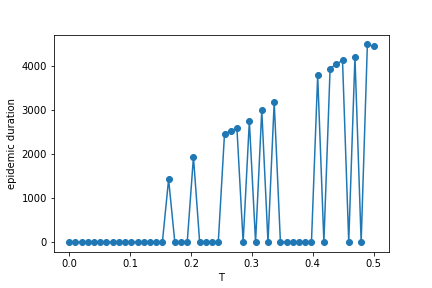
\includegraphics{../pics/tc_epilengths.png} \\
        Figure 1: Epidemic lengths for $T$ between 0 and 0.5.
    \end{center}}
    \Subproblem{The critical fraction $v_c$ to vaccinate for $T = 0.4$.}
    \Solution{I again selected the first of the set of generated graphs and chose the same node that I knew to be in the giant component to be the source of the epidemics. Then, for 50 values of $v$ between 0 and 1, I ran epidemics with transmissibility $(1-v)T$ for $T = 0.4$ and recorded the length of each epidemic. These results are plotted in Figure 2 below. After $v = 0.408$, epidemics no longer happen, so $v_c = 0.408$. 
    
    \begin{center}
        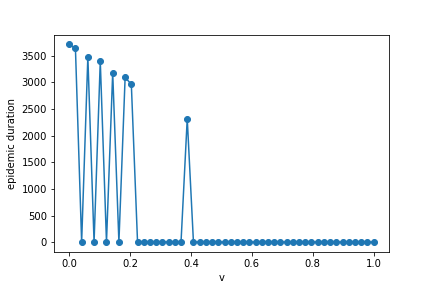
\includegraphics{../pics/vc_epilengths.png} \\
        Figure 2: Epidemic lengths for $v$ between 0 and 1.
    \end{center}}

    \Problem{Discrete-time SIR}{Run a discrete-time SIR model on a graph from the previous item starting from a single infecting node. Assume that each infecting node remains infecting for one time step. Plot the fraction of infecting nodes against time. Repeat 100 times. Make a prediction for how the duration of the epidemic scales with the number of nodes in the graph. What is the relationship between this SIR model and a breadth-first search?}
    \Solution{I coded the discrete-time SIR model based on the breadth-first search code I used for Homework 6. A discrete-time SIR model is simply breadth-first search with each color corresponding to a different compartment: susceptible individuals are the white nodes, infecting individuals are the gray nodes, and recovered individuals are the black nodes. As such, I was able to easily make two modifications to my breadth-first search code in order to transform it into a discrete-time SIR model. 
    
    The first and most important modification is that each vertex only gets visited in the innermost loop if a random probability is drawn below the prescribed transmissibility probability (here, this was $T = 0.4$). Where in BFS every node gets visited that's adjacent to each vertex, in a discrete-time SIR model this probability affects what nodes get infected. The second modification was that I removed the functionality that recorded path lengths and replaced it with a running calculation of the number of gray (infecting) nodes at each time step. In this way, the discrete-time SIR code naturally returns an array of the fraction of infecting individuals over time, making analysis easy.

    I generated a random graph in MATLAB with $n = 10^4$ nodes and ported the data into Python for analysis. After running the discrete-time SIR on 100 random nodes in the graph, I plotted all the infecting fractions over time overlaid on top of each other on the same figure (Figure 3 below). This creates a sort of pseudo-average, smoothing out the effects of all the different nodes and ignoring any infections which started on disconnected (non-giant) components. To me, it looks like this epidemic peters out around time step 1000 and does not last in a significant portion of the population (under 0.25\%) after this time step. As such, I predict that duration of the epidemic scales roughly like $n^3 \log n$ in the worst case and closer to $n^2\log n$ for the bulk of the population, judging by the sharp drop around time step 350 to 400 in Figure 3.

    \begin{center}
        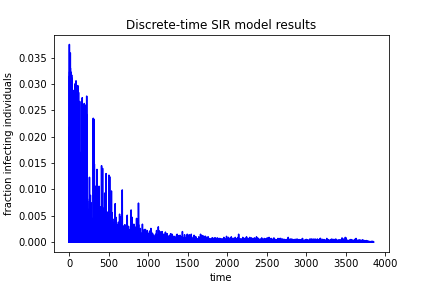
\includegraphics{../pics/discSIR.png} \\
        Figure 3: Discrete-time SIR model results. 
    \end{center}}

\end{document}